\documentclass{article}
\usepackage[utf8]{inputenc}
\usepackage{amsmath}
\usepackage{amssymb}
\usepackage{indentfirst}
\usepackage{color}
\usepackage{forest}
\usepackage{fancyhdr}
\usepackage{algorithm}
\usepackage[noend]{algpseudocode}
\usepackage{geometry}
\usepackage[T1]{fontenc}
\geometry{left=2.5cm,right=2.5cm,top=2.5cm,bottom=2.5cm}

\title{6.046/18.410 Problem Set 7}
\author{Yijun Jiang\vspace{3pt}\\Collaborator: Hengyun Zhou, Eric Lau}
%\email{yjjiang@mit.edu}
\date{\today}

\pagestyle{fancy}
\lhead{Yijun Jiang}
\rhead{6.046/18.410 Problem Set 7}

\begin{document}
\maketitle

\section{Solving a Geology Problem Set}
\subsection{Part (a)}
\subsubsection{$\textsc{Box-Packing}(A,M)$}
\noindent\textbf{Proof}:

We assume $m\leqslant n$, otherwise the extra $m-n$ boxes are unnecessary and we can reformulate the problem to $m=n$. Then the input size is $|x|=|(A,m)|=\Theta(n)$.

We design a verification algorithm $V_{BP}(x,y)=V_{BP}((A,m),y)$. The certificate $y$ is a partition of $A$ into $m$ subsets (allowing empty subsets), such that the sum of each group does not exceed unity. The certificate size is $|y|=O(m+n)=O(n)$, which is a polynomial of $|x|$.

$V_{BP}$ works as follows. (1) Check if $y$ contains $m$ subsets and if the union of these subsets equals $A$. (2) Sum over each group and check if all $m$ sums are no greater than unity. If both checks are passed, return YES. Otherwise, return NO.

Check (1) costs at most $O(n^2)$ time to identify the union of all subsets with $A$ (naively check every element against $A$). I can do better than $O(n^2)$, but I will not bother because I just want something polynomial. Check (2) costs $O(n)$ time because $O(n)$ additions and $O(m)$ comparisons are performed, and $m\leqslant n$ is assumed. Overall, the runtime of $V_{BP}$ is $O(n^2)$, which is a polynomial of $|x|$. In conclusion, \textsc{Box-Packing} is in NP.

%If we assume that $y$ is a proper partition of $A$, the first check is unnecessary. It is the second check that matters. However, this makes no difference since $V_{BP}$ runs in polynomial time anyway.

\subsubsection{$\textsc{Equal-Weight}(B)$}
\noindent\textbf{Proof}:

The input size is $|x|=|B|=\Theta(n\log(\max_ib_i))$. Note: here we assume that $b_i$ can be large, and all $b_i$ are represented by $\log(\max_ib_i)$ bits. If we do not take this into account, then $|x|=\Theta(n)$, and in the following discussion simply remove all $\log(\max_ib_i)$ terms. This does NOT affect the final conclusion of polynomial verification. And the reason why we do not assume large $a_i$ in the previous part is that, from the problem, $a_i$ should be on the same or lower order of the capacity of a box.

We design a verification algorithm $V_{EW}(x,y)=V_{EW}(B,y)$. The certificate $y$ is a partition of $B$ into 2 subsets, such that the sum of the first group equals the sum of the second. The certificate size is $|y|=O(n\log(\max_ib_i))$, which is a polynomial of $|x|$.

$V_{EW}$ works as follows. (1) Check if $y$ contains 2 subsets and if the union of these subsets equals $B$. (2) Sum over the first group and the second group, and check if both sums are equal. If both checks are passed, return YES. Otherwise, return NO.

Check (1) costs at most $O(n^2\log(\max_ib_i))$ time to identify the union of both subsets with $B$ (naively check every element against $B$). Check (2) costs $O(n\log(\max_ib_i))$ time because $O(n)$ additions are performed, each of which taking up $O(\log(\max_ib_i))$ time. Overall, the runtime of $V_{EW}$ is $O(n^2\log(\max_ib_i))$, which is a polynomial of $|x|$. In conclusion, \textsc{Equal-Weight} is in NP.

\subsubsection{$\textsc{Desired-Weight}(C,w)$}
\noindent\textbf{Proof}:

The input size is $|x|=|(C,w)|=\Theta(n\log(\max_ic_i)+\log w)$.

We design a verification algorithm $V_{DW}(x,y)=V_{DW}((C,w),y)$. The certificate $y$ is a subset of $C$, such that the sum of this subset equals $w$. The certificate size is $|y|=O(n\log(\max_ic_i))$, which is a polynomial of $|x|$.

$V_{DW}$ works as follows. (1) Check if $y$ is a subset of $C$. (2) Sum over this subset and check if the sum equals $w$. If both checks are passed, return YES. Otherwise, return NO.

Check (1) costs at most $O(n^2\log(\max_ic_i))$ time to verify a subset of $C$ (naively check every element against $C$). Check (2) involves $O(n)$ additions, each of which taking up $O(\log(\max_ic_i))$ time. And we do a comparison of $O(\log w)$. Overall, the runtime of $V_{DW}$ is $O(n^2\log(\max_ic_i)+\log w)$, which is a polynomial of $|x|$. In conclusion, \textsc{Desired-Weight} is in NP.

\subsection{Part (b)}
\subsubsection{$\textsc{Desired-Weight}\leqslant_p\textsc{Equal-Weight}$}
\noindent\textbf{Proof}:

The input $x=(C,w)$ for \textsc{Desired-Weight} has size $|x|=\Theta(n\log(\max_ic_i)+\log w)$. Given $x$, we design a reduction function $R(x)$ that returns an input $x'=B$ for \textsc{Equal-Weight} as follows. Let $w'=\sum_ic_i$. If $w'\geqslant2w$, $R(x)$ returns $B=C\cup\{w'-2w\}$. Otherwise, $R(x)$ returns $B=C\cup\{2w-w'\}$. By dividing into 2 cases, we guarantee that we do not add a negative weight. $R(x)$ involves $n$ additions, each of which taking up $O(\log(\max_ic_i))$ time. Also, $\log w$ work is done for the new element. Therefore, $R(x)$ runs in $O(n\log(\max_ic_i)+\log w)$ time, which is a polynomial of $|x|$. Moreover, $|R(x)|=O(n\log\max_i(c_i)+\log w)$ is a polynomial of $|x|$.

In order to reduce \textsc{Desired-Weight} to \textsc{Equal-Weight}, we need to prove that \textsc{Desired-Weight} returns YES if and only if \textsc{Equal-Weight} returns YES.

~

\noindent(1) $w'\geqslant2w$.

If $R(x)=B$ is a YES-input for \textsc{Equal-Weight}, there exists a partition of $B=C\cup\{w'-2w\}$ into two subsets, each of which sums up to $(\sum_ic_i+(w'-2w))/2=w'-w$. Say the newly added weight $w'-2w$ belongs to one subset $B_1$. Then the rest of $B_1$ sums up to $(w'-w)-(w'-2w)=w$. These rocks constitute the desired subset of $C$. Thus $x=(C,w)$ is a YES input for \textsc{Desired-Weight}.

On the other hand, if $x=(C,w)$ is a YES-input for \textsc{Desired-Weight}, there exists a subset $G$ of $C$ whose sum is $w$. Then $B_1=G\cup\{w'-2w\}$ and $B_2=B-B_1$ have the same sum $w'-w$. Thus $R(x)=B$ is a YES input for \textsc{Equal-Weight}.

\noindent(2) $w'<2w$

If $R(x)=B$ is a YES-input for \textsc{Equal-Weight}, there exists a partition of $B=C\cup\{2w-w'\}$ into two subsets, each of which sums up to $(\sum_ic_i+(2w-w'))/2=w$. Say the newly added weight $2w-w'$ belongs to one subset $B_1$. Then the other subset $B_2$ is the desired subset of $C$ that sums up to $w$. Thus $x=(C,w)$ is a YES input for \textsc{Desired-Weight}.

On the other hand, if $x=(C,w)$ is a YES-input for \textsc{Desired-Weight}, there exists a subset $G$ of $C$ whose sum is $w$. Then $B_1=G$ and $B_2=B-G$ have the same sum $w$. Thus $R(x)=B$ is a YES input for \textsc{Equal-Weight}.

~

This completes the proof that $\textsc{Desired-Weight}\leqslant_p\textsc{Equal-Weight}$. Since \textsc{Desired-Weight} is NP-complete and \textsc{Equal-Weight} is in NP, we conclude that \textsc{Equal-Weight} is NP-complete. Finally, notice that the only reason for us to consider whether $w'\geqslant2w$ is that, we are not informed if negative weights are allowed for \textsc{Equal-Weight}. If they are allowed, we do not need to divide $R(x)$ into two cases.

\subsubsection{$\textsc{Equal-Weight}\leqslant_p\textsc{Box-Packing}$}
\noindent\textbf{Proof}:

The input $x=B$ for \textsc{Equal-Weight} has size $|x|=\Theta(n\log(\max_ib_i))$. Given $x$, we design a reduction function $R(x)$ that returns an input $x'=(A,m)$ for \textsc{Box-Packing} as follows. Let $\alpha=2/\sum_ib_i$. Rescale $B'=[\alpha b_1,\alpha b_2,\cdots,\alpha b_n]$. Let $R(x)$ return $(A,m)=(B',2)$. $R(x)$ involves $n$ additions and rescalings, each of which taking up $O(\log(\max_ib_i))$ time. Therefore, $R(x)$ runs in $O(n\log(\max_ib_i))$ time, which is a polynomial of $|x|$. Moreover, say we keep $a_i=\alpha b_i$ to $\log(\max_ib_i)$ digits after the decimal point, then $|R(x)|=O(n\log(\max_ib_i))$ is a polynomial of $|x|$.

In order to reduce \textsc{Equal-Weight} to \textsc{Box-Packing}, we need to prove that \textsc{Equal-Weight} returns YES if and only if \textsc{Box-Packing} returns YES.

If $R(x)=(A,m)$ is a YES-input for \textsc{Box-Packing}, there exists a partition of $A=B'$ into $m=2$ subsets, such that the sum of each subset does not exceed unity. Since $\sum_ia_i=\alpha\sum_ib_i=2$, we conclude that both subsets sum up to exactly unity. This means that an equal-weight partition of $B'$ exists. Rescaling does not change this equality. Thus $x=B$ is a YES-input for \textsc{Equal-Weight}.

On the other hand, if $x=B$ is a YES-input for \textsc{Equal-Weight}, then there exist a partition $B=B_1\cup B_2$ such that $B_1$ and $B_2$ has the same sum. Correspondingly, there exist a partition $B'=B_1'\cup B_2'$ such that $B_1'$ and $B_2'$ has the same sum. Since $A=B'$ sums up to 2, $B_1'$ and $B_2'$ each sums up to unity. So they can be packed into $m=2$ boxes. Thus $R(x)=(A,m)$ is a YES-input for \textsc{Box-Packing}.

This completes the proof that $\textsc{Equal-Weight}\leqslant_p\textsc{Box-Packing}$. Since \textsc{Equal-Weight} is NP-complete and \textsc{Box-Packing} is in NP, we conclude that \textsc{Box-Packing} is NP-complete.

\subsection{Part (c)}
\noindent\textbf{Description}:

If $w>nk$, return NO. Otherwise, use dynamic programming. Let $D(i,v)$ be the answer to the following True/False question: is it possible to get weight $v\in\mathbb{Z}$ from a subset of $C_i=[c_1,c_2,\cdots,c_i]$? We construct a matrix of $D$ as stated in the next paragraph. In order to recover the desired subset, we also maintain a matrix $E$. $E(i,v)$ answers the following True/False question: if we do get weight $v\in\mathbb{Z}$ from a subset of $C_i$, do we need to use $c_i$?

Initially, set $D(0,0)=\textup{True}$ and $D(0,v)=\textup{False}$ for all $1\leqslant v\leqslant w$ (this is to make sure the edge cases are correct). Start from $i=1$ and do the following loop: use $D(i,v)=D(i-1,v)\textup{ OR }((v\geqslant c_i)\textup{ AND }D(i-1,v-c_i))$ to get $D(i,v)$ for all $0\leqslant v\leqslant w$. As we calculate $D(i,v)$, we also update $E(i,v)$: $E(i,v)=\textup{True}$ if and only if $D(i-1,v-c_i)=\textup{True}$ (when $v\geqslant c_i$). At the end of each iteration, increase $i$ by 1. Iterate until $i=n$. Return $D(n,w)$ as the solution to the decision problem (YES for True, NO for False). If the decision problem gives a YES answer, the search problem is solved by backwards tracing $E(i,v)$. Initially set $i=n$ and $v=w$. Iterate as follows. If $E(i,v)=\textup{True}$, store $c_i$ into $G$ and reduce $v$ by $c_i$. Otherwise keep $v$ unchanged. At the end of each iteration reduce $i$ by 1. When $i$ is reduced to zero, output $G$ as the desired subset. The details are shown in the pseudocode below.
\begin{algorithm}
\caption{Deside if the desired subset $G$ of $k$-bounded and interger-valued $C$ exists in polynomial time}
\begin{algorithmic}[1]
\Procedure{Decision-$k$-Bounded-Integer-Desired-Weight}{$C,w$}
\If{$w>nk$} \Return{False}
\Else{}
	\State{Create $(n+1)$-by-$(w+1)$ matrices $D$ and $E$}
	\State{$D(0,0)\gets\textup{True},E(0,0)\gets\textup{True}$}
	\For{$v=1:w$}
		\State{$D(0,v)\gets\textup{False},E(0,v)\gets\textup{False}$}
	\EndFor
	\For{$i=1:n$}
		\For{$v=0:w$}
			\If{$D(i-1,v)$}
				\State{$D(i,v)\gets\textup{True},E(i,v)\gets\textup{False}$}
			\ElsIf{$v\geqslant c_i$}
				\State{$D(i,v)\gets D(i-1,v-c_i),E(i,v)\gets D(i-1,v-c_i)$}
			\Else{}
				\State{$D(i,v)\gets\textup{False},E(i,v)\gets\textup{False}$}
			\EndIf
		\EndFor
	\EndFor
	\State\Return{$D(n,w),E$}
\EndIf
\EndProcedure

\Procedure{Search-$k$-Bounded-Integer-Desired-Weight}{$C,w$}
\State{$IfExist,E\gets$\Call{Decision-$k$-Bounded-Integer-Desired-Weight}{$C,w$}}
\If{$!IfExist$}\Comment{$(C,w)$ is a NO-input}
	\State{Raise exception: solution does not exist}
\Else{}\Comment{$(C,w)$ is a YES-input}
	\State{$G\gets[~],v\gets w$}
	\For{$i=n:-1:1$}
		\If{$E(i,v)$}
			\State{$G.append(C[i])$}
			\State{$v\gets v-C[i]$}
		\EndIf
	\EndFor
	\State{\Return{$G$}}
\EndIf
\EndProcedure
\end{algorithmic}
\end{algorithm}

~

\noindent\textbf{Correctness}:

If $w>nk$, it is impossible to find the desired subset, for the sum over entire $C$ is bounded above by $nk$. In the following discussion we focus on $w\leqslant nk$.

$D(i,v)$ is the possibility to get weight $v\in\mathbb{Z}$ from a subset of $C_i=[c_1,c_2,\cdots,c_i]$. There are two ways to make $D(i,v)=\textup{True}$. The first one is, if $D(i-1,v)=\textup{True}$, the desired subset for $C_{i-1}$ can be used as the desired subset of $C_i$. The second one is, if $v\geqslant c_i$ (so we can legally talk about $D(i-1,v-c_i)$) and if $D(i-1,v-c_i)=\textup{True}$, the desired subset for $C_{i-1}$, unioned with $\{c_i\}$, is the desired subset of $C_i$. Since by the time we iterate to $i$, all $D(i-1,v)$ is already calculated, we can obtain $D(i,v)$ for all $v$, where $v\leqslant w\leqslant nk$. When the iteration comes to $i=n$, we can get $D(n,w)$, which exactly indicates the existence of the desired subset $G$ for input $(C,w)$.

If the desired subset $G$ exists, we can write it out by backwards tracing $E(i,v)$. During the construction of $D$ and $E$, $E(i,v)$ is set True if and only if $D(i-1,v-c_i)=\textup{True}$. Therefore, $E(i,v)$ is True if and only if $c_i$ is selected as a member of the desired subset $G$. As a result, we can start from $i=n$ and $v=w$ and trace backwards. $E(i,v)=\textup{False}$ implies that $c_i\notin G$, so we should reduce $i$ and keep $v$. $E(i,v)=\textup{True}$ implies that $c_i\in G$, so we should reduce $i$ and reduce $v$ by $c_i$, and we store $c_i$. The existence of $G$ guarantees that we can reduce both $i$ and $v$ down to zero. Once that is done, all the elements of $G$ will be recovered.

This proves the correctness of the algorithm.

~

\noindent\textbf{Runtime}:

If $w>nk$, the algorithm terminates in constant time. Therefore, we focus on the case where $w\leqslant nk$. Notice that we loop over all $i\leqslant n$ and all $v$ where $v\leqslant w\leqslant nk$. Therefore, the runtime of the decision problem is $O(n^2k)$. If the decision problem answers YES, to find the solution $G$, $O(n)$ additional time is required, since we iterate $n$ times. Since $k$ is a constant, this is polynomial time of $n$, which is also polynomial time of the input size $\Theta(n+\log w)$. So the algorithm belongs to P.

\subsection{Part (d)}
\noindent\textbf{Description}:

Check the elements of $C$ one by one in reverse order. Instead of a loop, we recursively call \textsc{Superincreasing-Desired-Weight} to achieve this. As we recurse, we shorten $C$ by removing its last element and reduce $w$ if possible. Specifically, let the last element of $C$ be $c$. If $w\geqslant c$, we recurse on $(C-\{c\},w-c)$. Otherwise, we recurse on $(C-\{c\},w)$. The base cases are $w=0$ and $w\neq0,C=[~]$. In the first case, the desired subset exists and we output YES. In the second case, the desired subset does not exist and we output NO. The details are shown in the pseudocode below.
\begin{algorithm}
\caption{Deside if the desired subset $G$ of super-increasing $C$ exists in polynomial time}
\begin{algorithmic}[1]
\Procedure{Superincreasing-Desired-Weight}{$C,w$}
\If{$w=0$} \Return{True}
\ElsIf{$C=[~]$} \Return{False}
\Else{}
	\State{$c\gets C[end]$}
	\State{Remove the last element from $C$}	
	\If{$w\geqslant c$} {\Return\Call{Superincreasing-Desired-Weight}{$C,w-c$}}
	\Else{} {\Return\Call{Superincreasing-Desired-Weight}{$C,w$}}
	\EndIf
\EndIf
\EndProcedure
\end{algorithmic}
\end{algorithm}

~

\noindent\textbf{Correctness}:


We first prove that $c_i>\sum_{j=1}^{i-1}c_j$ for all $i$. Notice that $C$ has the property $c_{i-1}<c_i/2$ for all $i$. Therefore, $c_{i-k}<2^{-k}c_i$. Then $\sum_{j=1}^{i-1}c_j<\sum_{j=1}^{i-1}2^{-(i-j)}c_i=c_i(1-2^{-(i-1)})<c_i$.

We claim that the YES/NO answer in one recursion (not the base case) is the same as the answer in the subsequent recursion. The proof goes as follows.

Say in a resursion, $C$ has been shortened to $C_i=\{c_1,c_2,\cdots,c_i\}$, and $w$ has been reduced to $w_i$. If there is a subset $G_i$ in $C_i$ such that the sum over $G_i$ is $w_i$, if $c_i>w_i$, then $c_i\notin G_i$. Therefore $G_i\subset C_i-\{c_i\}$, which means that the following recursion, where $C_{i-1}=C_i-\{c_i\}$ and $w_{i-1}=w_i$, has a YES answer. If $c_i\leqslant w_i$, then $c_i\in G_i$, because otherwise $G_i$ can only contain elements in $C_i-\{c_i\}$, whose sum is $\sum_{j=1}^{i-1}c_j<c_i\leqslant w_i$, which leads to a contradiction. The rest of $G_i$ comes from $C_i-\{c_i\}$ and sums up to $w_i-c_i$. Therefore, in the subsequent recursion, where $C_{i-1}=C_i-\{c_i\}$ and $w_{i-1}=w_i-c_i$, there is a desired subset $G_{i-1}$.

On the other hand, if in a recursion there is a subset $G_i$ in $C_i$ such that the sum over $G_i$ is $w_i$, then in the previous recursion, if $c_{i+1}>w_{i+1}$, then $w_{i+1}=w_i$ and $G_{i+1}=G_i$; if $c_{i+1}\leqslant w_{i+1}$, then $w_{i+1}=w_i+c_{i+1}$ and $G_{i+1}=G_i\cup\{c_{i+1}\}$. In both cases we can construct a desired subset for the previous recursion.

Thus, the proof is done for both directions. So we can reduce the original YES/NO problem down to base cases. If $w_{base}=0$, then $G_{base}=[~]$ is the desired subset and we return True. This means that for the original input $(C,w)$, there is a desired subset $G$. The answer is YES and we do output YES. On the other hand, if $w_{base}\neq0$ and $C_{base}=[~]$, a desired subset $G_{base}$ does not exist and we return False. This means that for the original input $(C,w)$, there is no such desired subset $G$. The answer is NO and we do output NO. Consequently, the algorithm \textsc{Superincreasing-Desired-Weight} is correct.

~

\noindent\textbf{Runtime}:

The algorithm has $n$ iterations. In each iteration, operations on $c_i$ and $w_i$ costs $O(\log(\max_ic_i)+\log w)$ time. Therefore, the overall runtime is $O(n\log(\max_ic_i)+n\log w)$, which is a polynomial of the input size $|x|=n\log(\max_ic_i)+\log w$.

\subsection{Part (e)}
\noindent\textbf{Description}:

First we call $\textsc{Decision-Desired-Weight}(C,w)$. If it returns False, the algorithm terminates (we do NOT run \textsc{Search-Desired-Weight} described below), saying that such a valid subset $G$ does not exist. If it returns True, then such a valid subset $G$ exists and we can get $G$ by calling the following $\textsc{Search-Desired-Weight}(C,w)$. We remove elements from $C$ one by one, and each time use \textsc{Decision-Desired-Weight} to check if this removed element belongs to the desired subset $G$. The details are shown in the pseudocode below.
\begin{algorithm}
\caption{Search the desired subset $G$ of $C$ in polynomial time}
\begin{algorithmic}[1]
\Procedure{Search-Desired-Weight}{$C,w$}
\State\Comment{Only works if the desired subset exists: need to check by \textsc{Decision-Desired-Weight} first!}
\State{$G\gets[~]$}
\If{$C\neq\varnothing$}
	\State{$c\gets C[1]$}
	\State{Remove $C[1]$ from $C$}\Comment{Suppose labeling starts from 1}
	\State{$IfDiscard\gets\textsc{Decision-Desired-Weight}(C,w)$}
	\If{$IfDiscard$}
		\State{$G.append(\Call{Search-Desired-Weight}{C,w})$}
	\Else{}
		\State{$G.append(c)$}
		\State{$G.append(\Call{Search-Desired-Weight}{C,w-c})$}
	\EndIf
\EndIf
\State\Return{$G$}
\EndProcedure
\end{algorithmic}
\end{algorithm}

~

\noindent\textbf{Correctness}:

We prove that if a desired subset $G$ exists, \textsc{Search-Desired-Weight} finds such a $G$ (there can be multiple such subsets and one of them is returned). The existence of such a $G$ is checked by calling $\textsc{Decision-Desired-Weight}(C,w)$ beforehand. In the proof below we assume this decision problem outputs YES.

The algorithm recursively calls itself. In each recursion, $C$ is shortened and $w$ is reduced if possible. Say in the $i$-th recursion $C=C_i=\{c_i,c_{i+1},\cdots,c_n\}$ and $w=w_i$. We claim that for each $i$, at the start of the $i$-th recursion, $C_i$ has a desired subset $G_i$ that sums up to $w_i$. This is proved by induction.

This claim is guaranteed by the YES answer of \textsc{Decision-Desired-Weight} at the beginning. Now suppose the claim is correct for the $i$-th recursion. In this recursion, we remove $c_i$ to get $C_{i+1}$. If \textsc{Decision-Desired-Weight} outputs YES ($IfDiscard=\textup{True}$), we can find the desired subset without using $c_i$. So in the next recursion there is a subset of $C_{i+1}$ that sums up to $w_{i+1}=w_i$. On the other hand, if \textsc{Decision-Desired-Weight} outputs NO ($IfDiscard=\textup{False}$), we conclude that to reach a sum of $w_i$, the desired subset exists with $c_i$ and does not exist without $c_i$. So $c_i$ must be in the desired subset. The rest of $G_i$ sums up to $w_i-c_i$. So in the next recursion there is a subset of $C_{i+1}$ that sums up to $w_{i+1}=w_i-c_i$. In both cases, the claim continues to hold in the next recursion. Therefore, the claim holds for all $i$.

Moreover, if $w_i$ is reduced to $w_i-c_i$ in the $i$-th recursion, then the desired subset $G_i$ is obtained by appending $c_i$ to the desired subset $G_{i+1}$ in the $(i+1)$-th iteration. This is obvious since the sum over $G_{i+1}$ is $w_{i+1}=w_i-c_i$. On the other hand, if $w_i$ is not reduced in the $i$-th recursion, we can simply take $G_{i+1}$ as $G_i$. Therefore, we can construct the desired subset from the result of the deeper-level recursion. In the base case where $C_{base}=[~]$, obviously $G_{base}=[~]$. By returning to upper and upper recursion levels, this desired subset grows until its sum reaches $w$ in the first call of \textsc{Search-Desired-Weight}. Thus the algorithm is correct.

~

\noindent\textbf{Runtime}:

We focus on the case where the initial check $\textsc{Decision-Desired-Weight}(C,w)$ returns True, otherwise the algorithm terminates in constant time. In this case, \textsc{Search-Desired-Weight} is recursed $n$ times since each recursion reduces the size of $C$ by 1. Suppose the list-to-list appending operation only involves moving around constant number of pointers and thus costs constant time. Also \textsc{Decision-Desired-Weight} runs in constant time. Operations on $c$ and $w$ run in $O(\log(\max_ic_i)+\log w)$ time. Therefore, each recursion costs $O(\log(\max_ic_i)+\log w)$ time. The overall runtime is $O(n\log(\max_ic_i)+n\log w)$, which is a polynomial of the input size $|x|=n\log(\max_ic_i)+\log w$.

\section{Variants of Max Flow}
\subsection{Part (a): \textsc{Swap-Flow}}
\noindent\textbf{Proof}:

\noindent(1) Decision version of \textsc{Swap-Flow}

Instead of finding the maximum flow across all valid capacity functions, we are given an input $g>0$ and the YES/NO question is, does a valid capacity function $c$ exist such that the maximum flow $|f|$ is no less than $g$?

~

\noindent(2) Construction of a reduction function $R(x)$

For more readibility, an example of this construction is shown in Fig.\ref{example}.
\begin{figure}[!htbp]
	\centering
	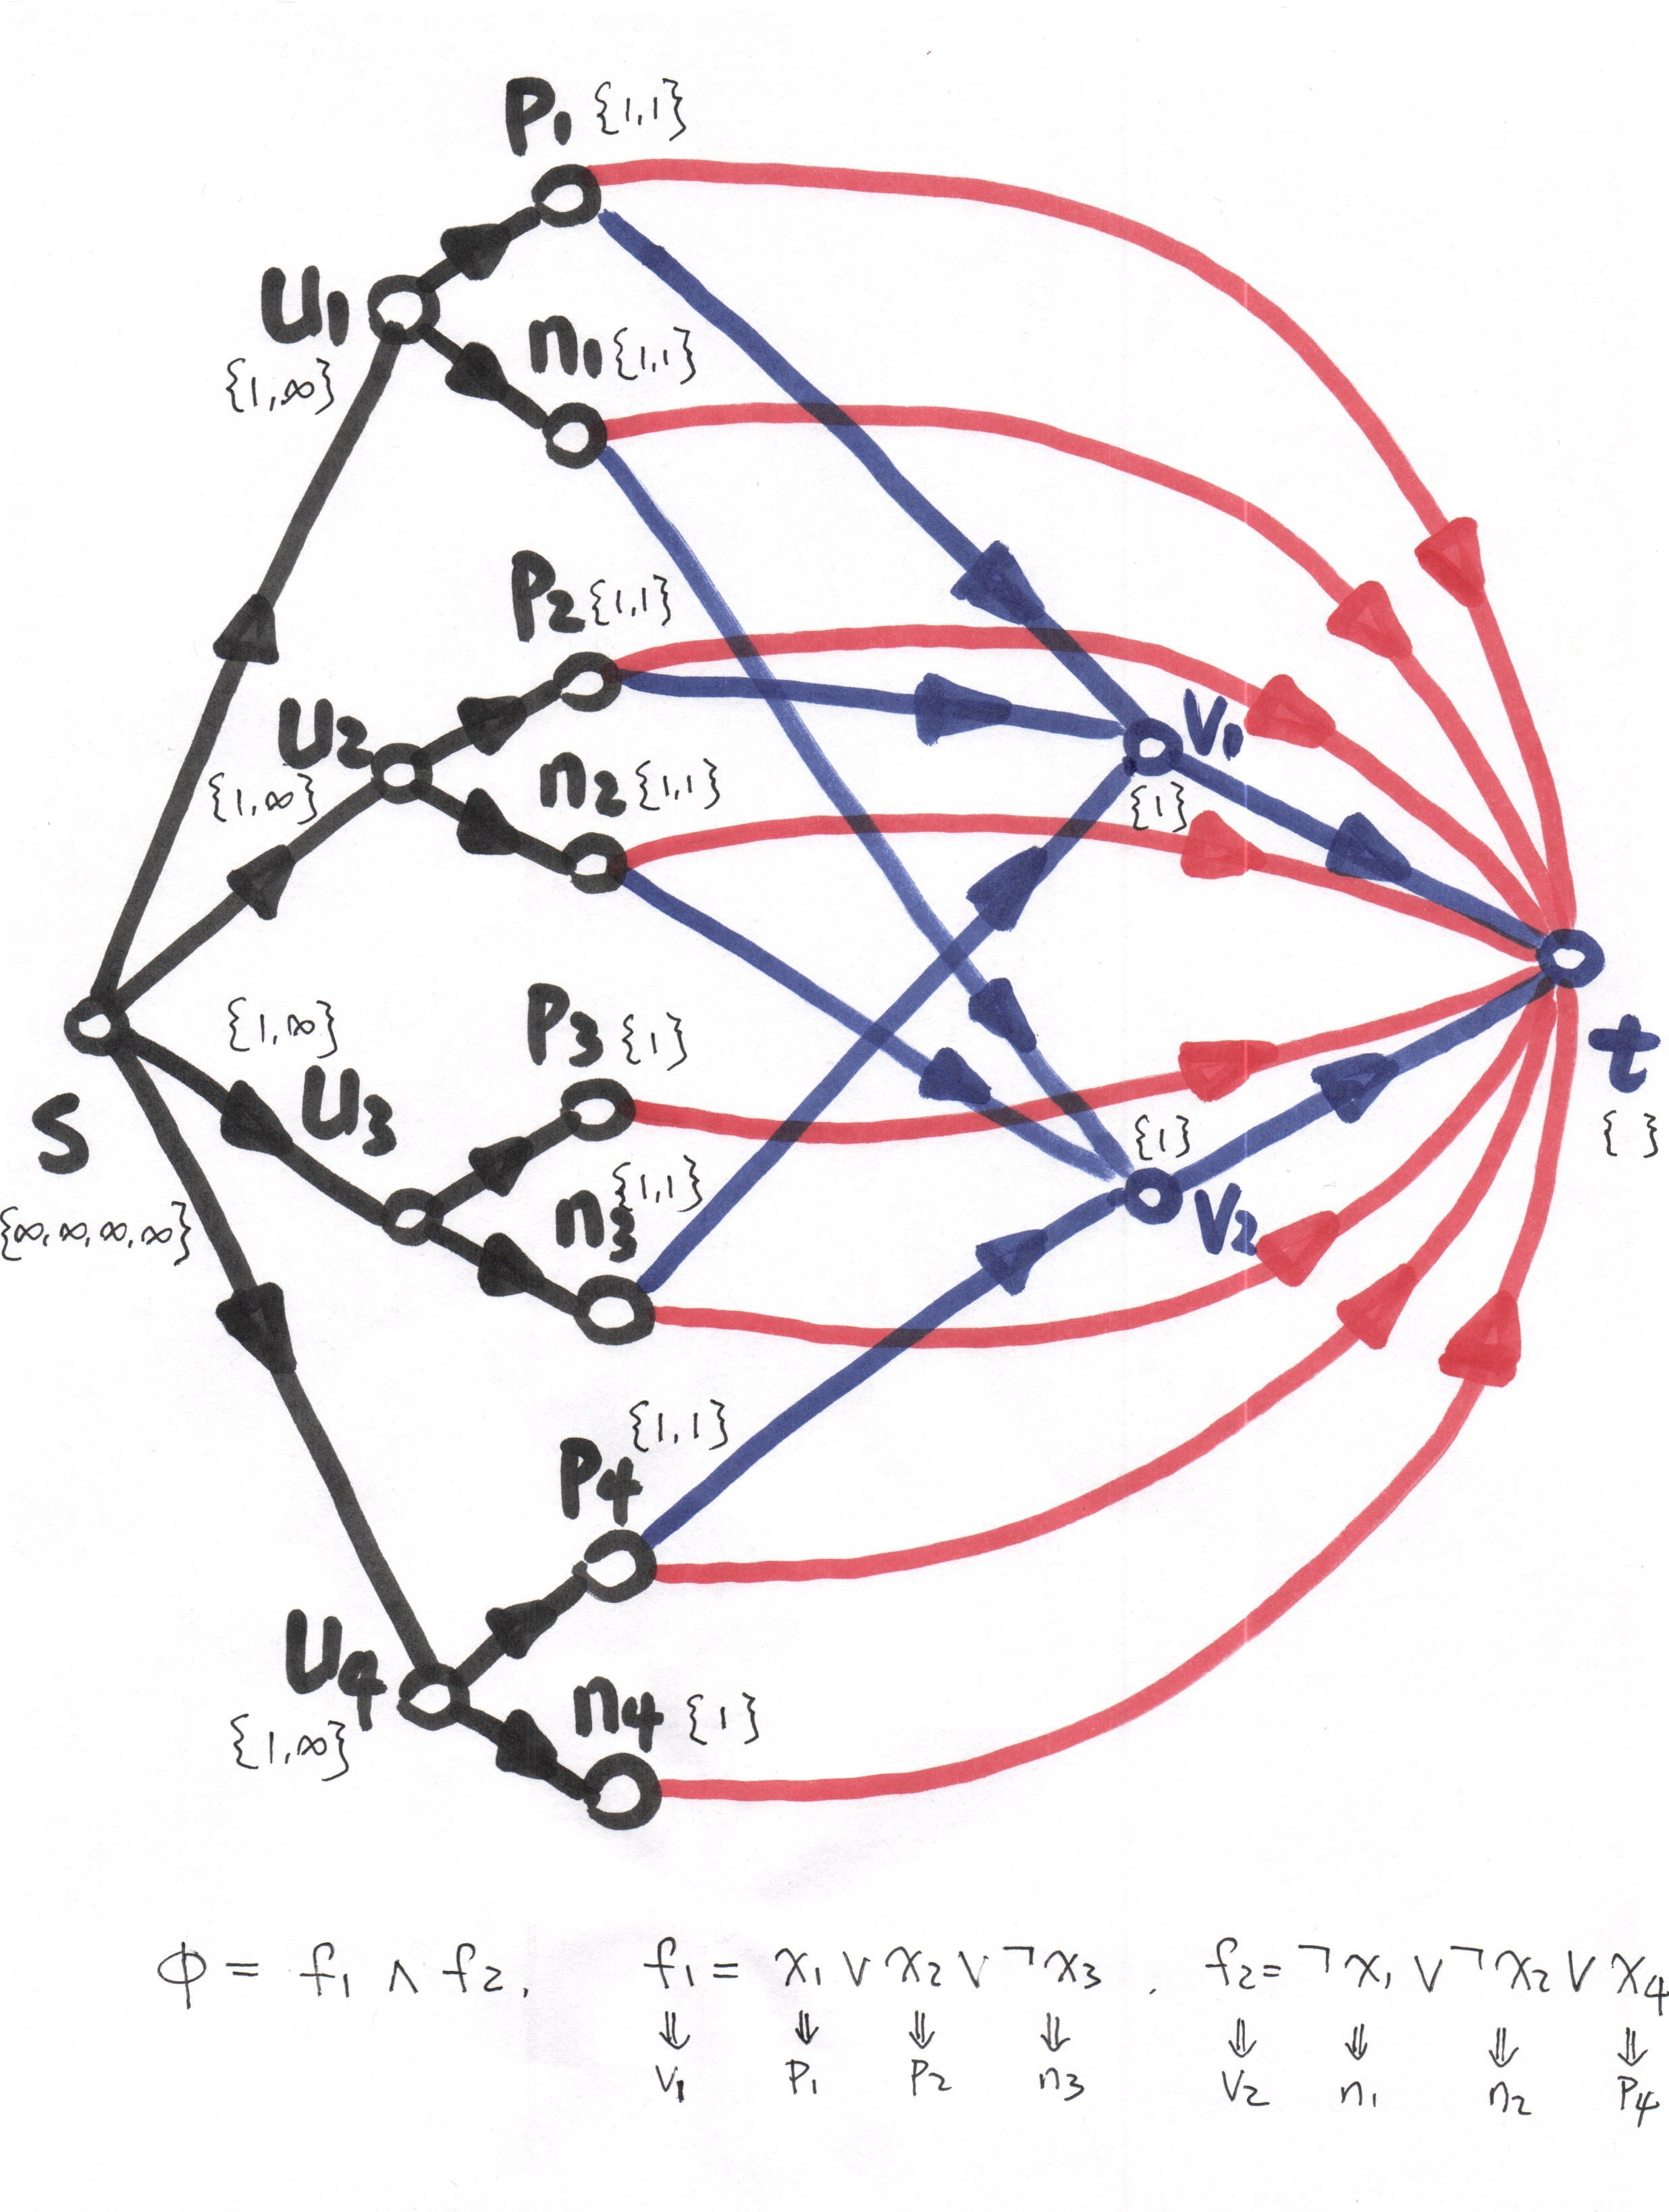
\includegraphics[width=10cm]{figure.jpg}\\
	\caption{A colored diagram of $R(x)$, i.e., an input for \textsc{Swap-Flow}, where $x=\phi=\mathfrak{f}_1\wedge\mathfrak{f}_2=(x_1\vee x_2\vee\neg x_3)\wedge(\neg x_1\vee\neg x_2\vee x_4)$ is an input for \textsc{3-SAT}.}
	\label{example}
\end{figure}

Given an input $x=\phi$ for \textsc{3-SAT}, we design a reduction function $R(x)$ that returns an input $x'=(G,C,g)$ for \textsc{Swap-Flow} as follows. Suppose $\phi$ contains $m$ clauses $\mathfrak{f}_1,\mathfrak{f}_2,\cdots,\mathfrak{f}_m$ and $n$ variables $x_1,x_2,\cdots,x_n$. By definition, $n\leqslant 3m$. So the input size is $|x|=O(m)$. Let $g=m+2n$. Now construct $G$ and $C$ as follows.

For each variable $x_i$, create three vertices: $p_i$ corresponding to the literal $x_i$, $n_i$ corresponding to the literal $\neg x_i$, and a third vertex $u_i$. Create directed edges $(u_i,p_i)$ and $(u_i,n_i)$. $u_i$ will not have any other outgoing edges. The idea is, $u_i$ can either flow to $p_i$ or to $n_i$, which stands for $x_i=\textup{True}$ or False. So ideally we would set $C(u_i)=\{0,\infty\}$. But the problem forbids it: $C(u_i)$ is required to be a set of POSITIVE integers. Then we must let $C(u_i)=\{1,\infty\}$ and deal with the additional unit capacity. For each $i\leqslant n$, we connect $p_i$ and $n_i$ directly to $t$ by edges $(p_i,t)$ and $(n_i,t)$ to get rid of this additional unit of flow. As we see in the following, $c(p_i,t)=c(n_i,t)=1$ by a good choice of $C$.

Create $(s,u_i)$ for all $i\leqslant n$. $s$ does not connect to any other vertices. Let $C(s)=\{\underbrace{\infty,\infty,\cdots,\infty}_n\}$. This guarantees that for any valid capacity function, $c(s,u_i)=\infty$. Technically speaking, $C(s)$ not a set since there are duplicate entries. But it is reasonable to assume that we are not required to use a rigorous set.

For each clause $\mathfrak{f}_j$, create a vertice $v_j$. If $x_{j_\alpha}$ or $\neg x_{j_\alpha}$ appears in $\mathfrak{f}_j$, create an edge $(p_{j_\alpha},v_j)$ or $(n_{j_\alpha},v_j)$, where $\alpha=1,2,3$. Also, create the only outgoing edge from $v_j$, which is $(v_j,t)$. Let $C(v_j)=\{1\}$.

For each $p_i$ or $n_i$, count its out-degree (denoted by $d$). Let $C(p_i)=\{\underbrace{1,1,\cdots,1}_{d_{p_i}}\}$ and $C(n_i)=\{\underbrace{1,1,\cdots,1}_{d_{n_i}}\}$. This guarantees that for any valid capacity function, $c(p_{j_\alpha},v_j)=1$ (or $c(n_{j_\alpha},v_j)=1$ if it is $\neg x_{j_\alpha}$ in clause $\mathfrak{f}_j$) for all $j\leqslant m$ and $\alpha=1,2,3$. Moreover, $c(p_i,t)=c(n_i,t)=1$ for all $i\leqslant n$.

This completes the construction of $G$. Notice that by this construction, the sink $t$ has in-degree $g=m+2n$, for there are edges $(v_j,t)$ for all $j\leqslant m$, as well as $(p_i,t)$ and $(n_i,t)$ for all $i\leqslant n$. All incoming edges of $t$ have unit capacity for any valid capacity function. Therefore, the maximum flow cannot exceed $g$. The decision problem, in this context, is actually asking if this maximum flow can equal $g$.

The size and runtime of $R(x)$ are calculated here. $|V|=3n+m+2$ and $|E|=n+2n+3m+m=3n+4m$. So $|G|=O(|V|+|E|)=O(m+n)=O(m)$. The size of $C$ is $O(|E|)=O(m+n)=O(m)$. The size of $g$ is $\log(m+2n)=O(\log m)$. Thus, the total size of $R(x)$ is $O(m)$, a polynomial of $|x|$. Each vertex and edge of $G$, as well as each element in $C(u)$ for each $u$, is created in constant time. So the runtime of $R(x)$ is linear with respect to its size. It is also $O(m)$, a polynomial of $|x|$.

~

\noindent(3) Equivalence of a YES-input $x$ and a YES-input $R(x)$

As the last step, we show that $x=\phi$ is a YES-input for \textsc{3-SAT} if and only if $R(x)=(G,C,g)$ is a YES-input for \textsc{Swap-Flow}.

~

First, if $R(x)=(G,C,g)$ is a YES-input for \textsc{Swap-Flow}, there exists a valid capacity function $c$ such that the maximum flow $f$ in $G$ satisfies $|f|\geqslant g=m+2n$. As is mentioned above, it is actually $|f|=g$ that holds. All the incoming edges of $t$ are saturated. i.e., $f(v_j,t)=c(v_j,t)=1$ for all $j\leqslant m$, and $f(p_i,t)=c(p_i,t)=1$, $f(n_i,t)=c(n_i,t)=1$ for all $i\leqslant n$.

Since all capacities are integers, according to CLRS (Theorem 26.10), there exists a maximum flow that is an integer flow. So WLOG suppose $f$ is an integer flow. For each $j\leqslant m$, since $f(v_j,t)=c(v_j,t)=1$, there must be unity flow along $(p_{j_\alpha},v_j)$ or $(n_{j_\alpha},v_j)$ for some $\alpha\leqslant3$. WLOG, let $f(p_{j_1},v_j)=1$. By construction, $x_{j_1}$ appears in clause $\mathfrak{f}_j$. We assign True to $x_{j_1}$, so that $\mathfrak{f}_j$ is satisfied. Similarly, if $f(n_{j_1},v_j)=1$, $\neg x_{j_1}$ appears in clause $\mathfrak{f}_j$ and we assign False to $x_{j_1}$.

By doing this assignment to all $j\leqslant m$, every clause $\mathfrak{f}_j$ is satisfied, and so is $\phi$. We claim that this assignment is self-consistent. This is because, say $f(p_{j_1},v_j)=1$ for some $j$ (which assigns True to $x_{j_1}$), we must have $f(u_{j_1},p_{j_1})\geqslant f(p_{j_1},v_j)+f(p_{j_1},t)=2$. Therefore, $c(u_{j_1},p_{j_1})\geqslant2$. Since $C(u_{j_1})=\{1,\infty\}$, it must be that $c(u_{j_1},p_{j_1})=\infty$ and $c(u_{j_1},n_{j_1})=1$. $n_{j_1}$ cannot flow to any $v_{j'}$ because $f(n_{j_1},t)=1$ has taken up this unit capacity. So $x_{j_1}$ will never be assigned False. Similarly, if $x_{j_1}$ is assigned False, it will never be assigned True again.

After this procedure, there may be some $x_i$ left unassigned. They can be assigned either to True of to False, for their values do not matter. The overall assignment satisfies $\phi$. Therefore, $x=\phi$ is a YES-input for \textsc{3-SAT}.

~

Next, we prove the opposite direction. If $x=\phi$ is a YES-input for \textsc{3-SAT}, there exists an assignment of True or False to $x_i$ for all $i\leqslant n$ such that clause $\mathfrak{f}_j$ is satisfied for all $j\leqslant m$. According to this assignment, we show that there is a valid capacity function $c$ for \textsc{Swap-Flow} that makes $|f|=g$. This capacity function is described as follows. For each $i$, if $x_i$ is assigned True, then $c(u_i,p_i)=\infty$ and $c(u_i,n_i)=1$. Otherwise, $c(u_i,p_i)=1$ and $c(u_i,n_i)=\infty$. For all other vertices, the swap is trivial: by construction of $R(x)$, it is guaranteed that any edge starting from $s$ has capacity $\infty$, and any edge starting from $p_i,n_i$ or $v_j$ has capacity 1, for all $i\leqslant n$ and $j\leqslant m$.

We show that under this capacity function, there is a flow $f$ such that $|f|=g$. First of all, consider the flow $f'$ such that $f'(s,u_i)=2$, $f'(u_i,p_i)=f'(p_i,t)=1$ and $f'(u_i,n_i)=f'(n_i,t)=1$ for all $i\leqslant n$. The other edges have zero flows. $f'$ satisfies $f'(e)\leqslant c(e)$ for every edge $e$ and flow conservation at every vertex. Therefore, $f'$ is a valid flow. $|f'|=2n$ since $(p_i,t)$ and $(n_i,t)$ with unit capacities are saturated for $i\leqslant n$.

Then we consider the flow $f''$ defined as follows. For each clause $\mathfrak{f}_j$, pick exactly one literal that is True. This can be done since $\phi$ is satisfiable. Say for $\mathfrak{f}_j$ the literal is $x_{j_\alpha}$. Let $f''(s,u_{j_\alpha})=f''(u_{j_\alpha},p_{j_\alpha})=f''(p_{j_\alpha},v_j)=f''(v_j,t)=1$. If, on the other hand, the literal is $\neg x_{j_\alpha}$, we simply replace $p_{j_\alpha}$ with $n_{j_\alpha}$ in the assignment above. For all other edges, set their flow to be zero. $f''$ satisfies $f''(e)\leqslant c(e)$ for every edge $e$ and flow conservation at every vertex. Therefore, $f''$ is a valid flow. $|f''|=m$ since $(v_j,t)$ with unit capacity is saturated for $j\leqslant m$.

Notice that, by choosing this capacity function, only edges with infinite capacities carry flows both in $f'$ and $f''$. Therefore, $f=f'+f''$ satiesfies $f(e)\leqslant c(e)$ for all edges $e$. Moreover, since flow conservation holds for both $f'$ and $f''$, it also holds for $f$. This means that $f$ is a valid flow in $G$, and $|f|=|f'|+|f''|=m+2n=g$. Therefore, $R(x)=(G,C,g)$ is a YES-input for \textsc{Swap-Flow}.

~

This completes the proof that $\textsc{3-SAT}\leqslant_p\textsc{Swap-Flow}$. Since \textsc{3-SAT} is NP-complete, we conclude that \textsc{Swap-Flow} is NP-hard.

\subsection{Part (b): \textsc{All-Or-None-Flow}}
\noindent\textbf{Proof}:

\noindent(1) Decision version of \textsc{All-Or-None-Flow}

Instead of finding the maximum flow under the restriction that $f(e)=0$ or $f(e)=c(e)$ for all edges $e$, we are given an input $g>0$ and the YES/NO question is, does a flow $f$ under this restriction exist such that $|f|\geqslant g$?

~

\noindent(2) Proof of $\textsc{All-Or-None-Flow}\in\textup{NP}$

The input is $x=(G,c(e),g)$, where $G=(V,E)$ is the flow network and $c(e)$ is the capacity function that assigns each edge a positive capacity. The input size is $|x|=\Theta(|V|+|E|+|E|\log(\max_ec(e))+\log g)$. Note: here we assume that $c(e)$ and $g$ can be large. If we do not take this into account, then $|x|=\Theta(|V|+|E|)$, and in the following discussion simply remove all $\log(\max_ec(e))$ and $\log g$ terms. This does NOT affect the final conclusion of polynomial verification.

We design a verification algorithm $V_{AONF}(x,y)=V_{ANOF}((G,c(e),g),y)$. The certificate $y$ is a flow $f$ over $G$ such that $f(e)=0$ or $f(e)=c(e)$ for all $e\in E$, and $|f|\geqslant g$ holds. The certificate size is $|y|=O(|E|\log(\max_ef(e)))=O(|E|\log(\max_ec(e)))$ because the flow is determined by its values on all edges. It is a polynomial of $|x|$.

$V_{ANOF}$ works as follows. (1) Check that $f(e)$ is either 0 or $c(e)$ for all $e\in E$. (2) Check that $|f|\geqslant g$. If both checks are passed, return YES. Otherwise, return NO.

Check (1) costs $O(|E|\log(\max_ec(e)))$ time because it loops over $E$ and in each loop an $O(\log(\max_ec(e)))$ comparason is done. Check (2) costs $O(|V|\log(\max_ec(e))+\log g)$ time if we use $|f|=\sum_uf(s,u)$ and compare $|f|$ with $g$. Overall, the runtime of $V_{ANOF}$ is $O(|V|\log(\max_ec(e))+|E|\log(\max_ec(e))+\log g)$, which is a polynomial of $|x|$. In conclusion, \textsc{All-Or-None-Flow} is in NP.

~

\noindent(3) Construction of a reduction function $R(x)$

The input $x=B=\{b_1,b_2,\cdots,b_n\}$ for \textsc{Equal-Weight} has size $|x|=\Theta(n\log(\max_ib_i))$. Given $x$, we design a reduction function $R(x)$ that returns an input $x'=(G,c(e),g)$ for \textsc{All-Or-None-FLow} as follows. Create a source $s$, a sink $t$ and an intermediate vertex $m$. Create $n$ edges from $s$ to $m$ (see my note for parallel edges in the subsequent paragraph). Label them as $e_{sm}^i$, where $i=1,2,\cdots,n$, and let $c(e_{sm}^i)=2b_i$. Also create $n$ edges from $m$ to $t$. Label them as $e_{mt}^i$, where $i=1,2,\cdots,n$, and let $c(e_{mt}^i)=b_i$. Let $g=\sum_ib_i$. $|R(x)|=O(|V|+|E|+|E|\log(\max_ib_i)+\log g)=O(n\log(\max_ib_i))$, which is a polynomial of $|x|$. The runtime of $R(x)$ is $O(|V|+|E|+n\log(\max_ib_i))=O(n\log(\max_ib_i))$, which is also a polynomial of $|x|$.

Note: by some definitions of flow network, we cannot have parallel edges between two vertices. This can be easily solved by adding an auxilliary vertex dividing each edge into two, both of the same capacity. Therefore, we will not worry about parallel edges in the following discussion.

In order to reduce \textsc{Equal-Weight} to \textsc{All-Or-None-Flow}, we need to prove that \textsc{Equal-Weight} returns YES if and only if \textsc{All-Or-None-Flow} returns YES.

~

\noindent(4) Proof of $\textsc{Equal-Weight}\leqslant_p\textsc{All-Or-None-Flow}$

If $R(x)=(G,c(e),g)$ is a YES-input of \textsc{All-Or-None-Flow}, there exists a flow $f$ such that $|f|\geqslant g$. By construction, $\sum_ic(e_{mt}^i)=\sum_ib_i=g$, so $|f|\leqslant g$. Therefore, it must be that $|f|=g$.

This means that $\sum_if(e_{sm}^i)=g$. Notice that $\sum_ic(e_{sm}^i)=\sum_i2b_i=2g$. Because $f$ is restricted such that $f(e)$ is either 0 or $c(e)$, we conclude that some edges between $s$ and $m$ are fully utilized and the others are empty. Let $B_1=\{b_j|e_{sm}^j\textup{ is fully utilized}\}$ and $B_2=B-B_1$. $\sum_{b_j\in B_1}2b_j=\sum_{b_j\in B_1}c(e_{sm}^j)=|f|=g$. Therefore, $B_1$ sums up to $g/2$, and so does $B_2$. This means that $B$ can be partitioned into two equi-sum subsets. Thus, $x=B$ is a YES-input for \textsc{Equal-Weight}.

On the other hand, if $x=B$ is a YES-input of \textsc{Equal-Weight}, there exists a partition of $B$ into two subsets, $B_1$ and $B_2$, such that the sum over $B_1$ equals the sum over $B_2$.

For each $j$ such that $b_j\in B_1$, we push $c(e_{sm}^j)=2b_j$ flow through the edge $e_{sm}^j$. All other edges between $s$ and $m$ are not used. This produces a total incoming flow of $\sum_{b_j\in B_1}2b_j=\sum_ib_i=g$ at vertex $m$. For all edges $e_{mt}^i$, we push $c(e_{mt}^i)=b_i$ flow through them. This produces a total outgoing flow of $\sum_ib_i=g$ at vertex $m$. Therefore, flow at $m$ is conserved. Moreover, this flow guarantees that each edge is either fully used or not used at all. Call this flow $f$. $f$ is a valid solution and $|f|=g$. Thus, $R(x)=(G,c(e),g)$ is a YES-input for \textsc{All-Or-None-Flow}.

~

This completes the proof that $\textsc{Equal-Weight}\leqslant_p\textsc{All-Or-None-Flow}$. Since \textsc{Equal-Weight} is NP-complete and \textsc{All-Or-None-Flow} is in NP, we conclude that \textsc{All-Or-None-Flow} is NP-complete.

\end{document}
